% Author: Magdalen Berns

\chapter{The Physiology of The Eye}

\label{anatomy}
\lhead{\emph{The Physiology of The Eye}}
\section{A Normal, Healthy Eye}

The human eye is a complex biological system, which allows the brain to
form an image of its surroundings through the interpretation of
electromagnetic signals. \Fref{fig:eye_simple} shows a simple schematic
diagram of the layout of the eye. The structure of the eye is designed to
project a focused image onto the the back of the retina so the light rays
can be converted into electrical signals which are passed to the brain by
the optic nerve.

\begin{figure}[!htbp]
\centering
  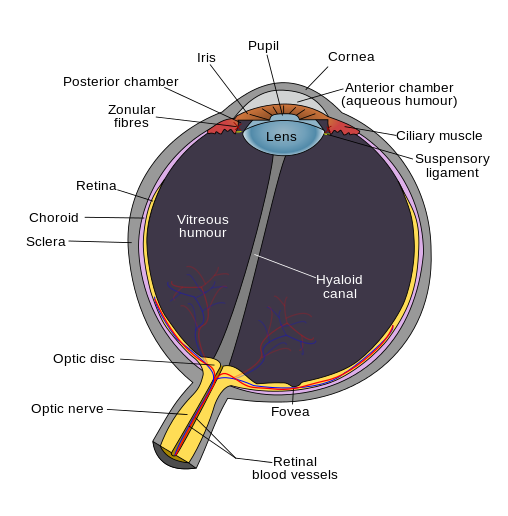
\includegraphics{figures/schematic_diagram_of_the_human_eye}
\caption{A simple schematic diagram of the layout of the eye.\cite{wikiRhcastilhos}}
\label{fig:eye_simple}
\end{figure}

The cornea of the eye is a transparent layer around 0.6mm thick
which curves around the iris as well as the anterior
chamber.\cite{yaylali1997corneal,thoft1983x,patel1994refractive}
With a mean refractive index of around 1.4 (about the same as water),
the cornea allows plenty of light to pass through. Incident light refracts
as in a convergent lens due to the convex shape of the cornea. 
\Eref{eq:refractive} shows Snell's Law of refraction for a light wave
passing through two different isotropic materials which have refractive
indices $n_1$ and $n_2$, respectively.

\begin{figure}[htbp]
\centering
  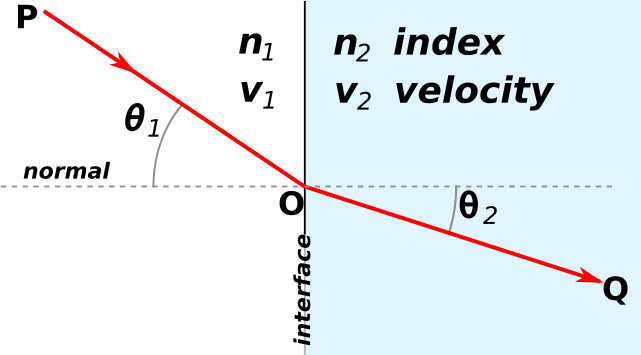
\includegraphics{figures/snells}
\caption{Snell's law for refraction at an interface where
             $n_1$ \textless $n_2$.\cite{wikisnell}}
\label{fig:snell}
\end{figure}

The angle $\theta_1$ is between the normal to the interface($n_1$ and $n_2$)
and the incident light ray and the angle $\theta_2$ is between the normal to
the interface($n_2$ and $n_1$) and the transmitted light ray, as shown in
\fref{fig:snell}.

\begin{equation}
n_1\sin\theta_1=n_2\sin\theta_2
\label{eq:refractive}
\end{equation}

The outermost surface of the cornea is made of epithelial cells which
are cyclically lost and replenished.
\cite{jester1999cellular,hassell2010molecular} The reproduction
of cells is facilitated in part by tear ducts, which serve to
moisten the eyes and remove harmful bacteria.\cite{holly1977tear}

There is a small circular opening in the iris (the coloured section of
the eye) called the pupil, which has an aperture of around 7mm that
dilates to allow an appropriate amount of light to pass through
the lens onto the retina.\cite{krugman1964some} As a consequence of
this optical setup the pupil acts as a diffraction grating, which places a 
fundamental limitation on visual resolution. 

The angular resolution, $\theta$ of the focal point on the retina is limited by
the diameter $D$ of the pupil and is directly proportional to the wavelength
of the diffracted light, $\lambda$ as expressed in the Rayleigh criterion
 \eref{eq:res_limit}.\cite{rayleigh1907dynamical}

\begin{equation}
\theta=\frac{1.22\lambda}{D}
\label{eq:res_limit}
\end{equation}

The optical resolution is the distance from the eye multiplied by the angular
resolution. The maximum achievable resolution of the eye corresponds to
$500nm$ so using \eref{eq:res_limit} with \eref{eq:eye_res}, $\theta=$.

\begin{equation}
\theta=\frac{1.22\times 500nm}{7mm}
\label{eq:eye_res}
\end{equation}

Following the initial refraction through the cornea, light is again refracted
through the lens to finely focus the image to a central point on the retina.
\Fref{fig:light_journey} illustrates the journey of light through the eye
onto the retina. The image on the retina is actually an upside down
projection of the original image, so it has to be translated by the brain.

\begin{figure}[!ht]
\centering
  \includegraphics{figures/light}
\caption{}
\label{fig:light_journey}
\end{figure}

The lens maker’s formula in \eref{eq:lens_makers} is an expression which relates the
focal point of a lens to the distance of the object and image from the lens centre,
as is illustrated in \fref{fig:convergent_lens}.

\begin{equation}
\frac{1}{S_1} + \frac{1}{S_2} = \frac{1}{f}
\label{eq:lens_makers}
\end{equation}

\begin{figure}[htbp]
\centering
  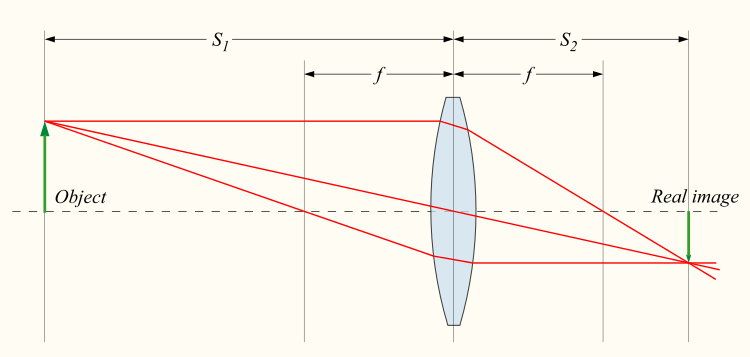
\includegraphics{figures/convergent_lens2}
\caption{The convex lens focuses the object(distance $S_1$ from the lens centre)
         and inverts this image(at a distance $S_2$ from the lens centre).
         \cite{greivenkamp2004field}}
\label{fig:convergent_lens}
\end{figure}

The lens is accommodated by a ciliary body of tissue which made up of fiber and
muscle. The ciliary body secretes a fluid, (known as aqueous humour) into a canal
that flows around the circumference of the eye, scleral venous sinus.
\cite{bill1970effects,dvorak1934schlemm} The primary function of the aqueous humour
is to maintain intraocular pressure by transferring fluids around the eye.

When the eye focuses on objects that are nearby, the ciliary body muscles contract,
causing the lens to flatten as a result of contractile forces. If an object is far
away the light rays can be approximated as parallel to the principal axis of the lens.
To focus on distant objects the suspensory ligaments relax to allow the lens to return
to a normal curved shape, hence light is refracted and focused onto the retina.

\begin{figure}[!htbp]
\centering
  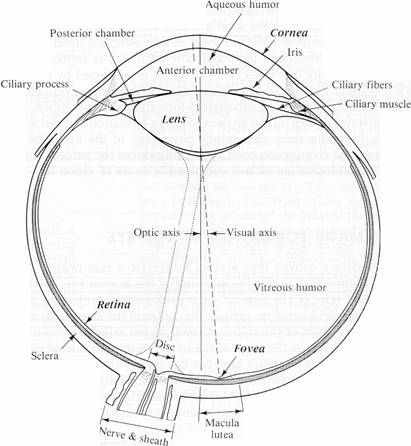
\includegraphics{figures/eye_diagram}
\caption{A diagram of the eye showing of the visual
 and optic axis, the cornea, the retina and the fovea}
\label{fig:optic_axis}
\end{figure}

Photons of light are refracted out of the lens before they pass through
a clear substance called the vitreous chamber and land onto the retina,
which is also transparent. A diagram indicating the optic axis and
visual axis is shown in \fref{fig:optic_axis}.

The retina is a membrane which covers the entire receptive field of
vision, it is part of the central nervous system.\cite{rogers1983neurite}
Just behind the retina are ganglion cells, biploar cells, cones and rods.
These are supported by pigment epithelium cells and the choroid - a
vascular bed of tissues which supply the retina with blood and removes
toxins. \cite{lutty1996localization} A schematic overview of the core
retinal constitution is given in \fref{fig:retina}

\begin{figure}[htbp]
\centering
  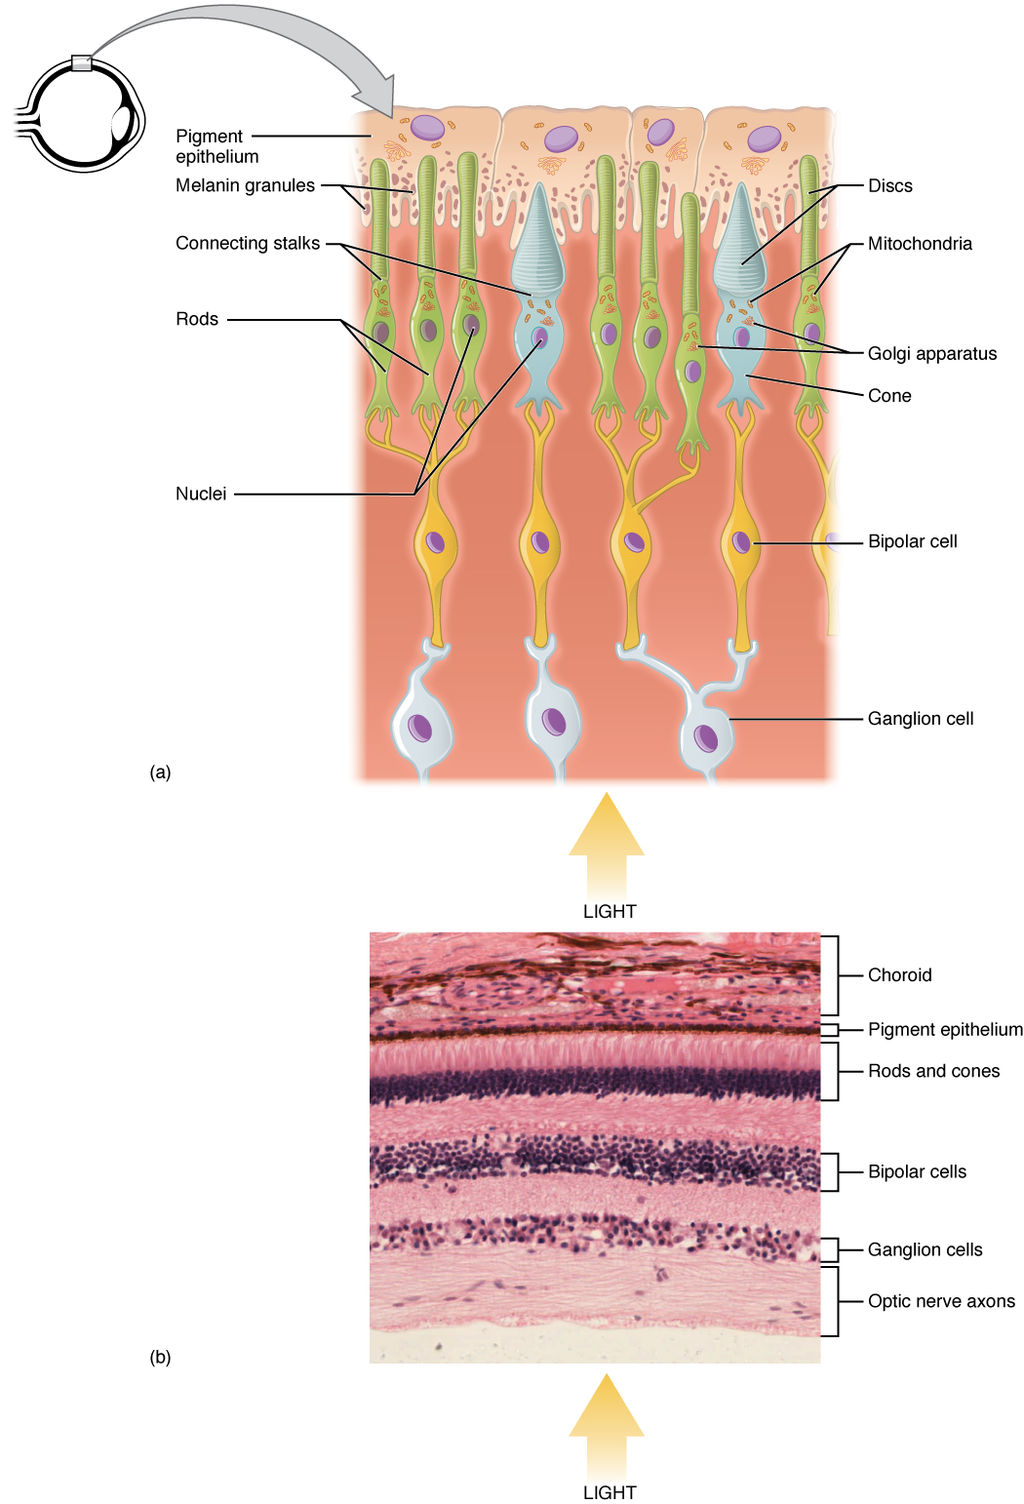
\includegraphics{figures/rods_and_cones}
\caption{A schematic diagram of the retina with the direction of light indicated
as being from the bottom upwards direction.}
\label{fig:retina}
\end{figure}

There are around 0.7 to 1.5 million ganglion cells in a normal human retina.
\cite{curcio1990topography}. Retinal ganglion cells are a form of neurons
and are integral in the transmission of electrical signals to the brain.
\cite{meyer1995characterization} Cones and rods are photoreceptors
that convert light into electrical signals which are transmitted to the
brain from the optic nerve, via bunches of ganglion nerves.

\begin{figure}[!htbp]
\centering
  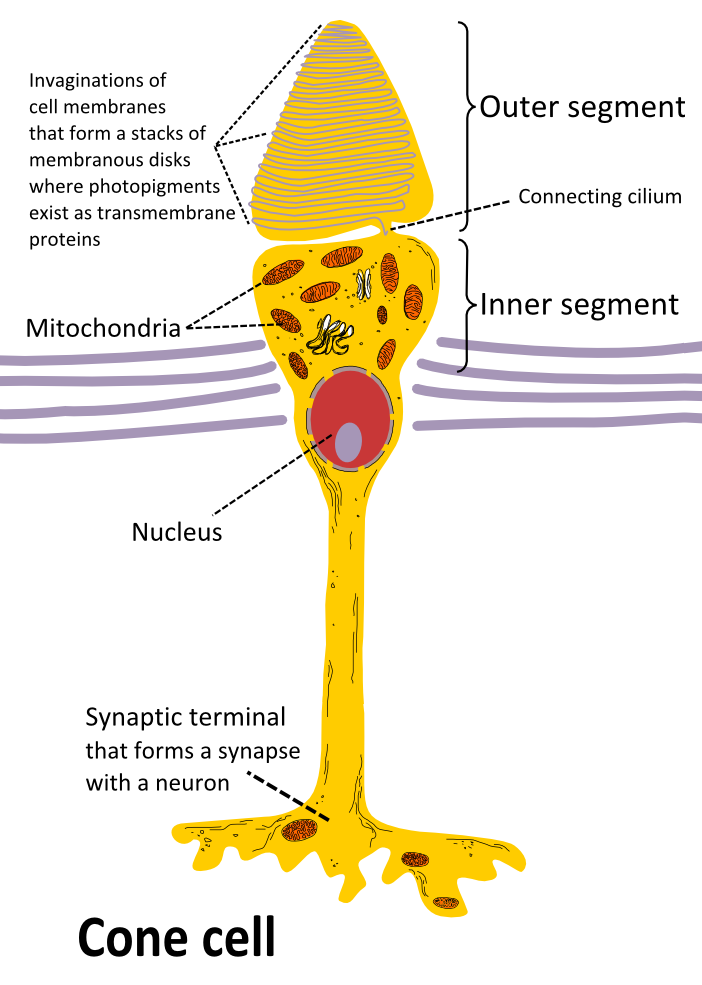
\includegraphics{cone_cell}
\caption{A schematic diagram of the cone cell showing the outer and inner
segments, nucleus and the synaptic terminal.\cite{wikicone}}
\label{fig:cone}
\end{figure}

Whilst cones are not particularly sensitive to light, they do aid to visual
acuity by granting us colour vision (\fref{fig:cone} shows a schematic
diagram of the cone cell).\cite{bowmaker1980visual} Conversely, rods
which have a region of pigments around $1\mu{m}$, are particularly
sensitive, even to the pressure exerted by a single photon of light. Rods
tend to be located around the periphery of the receptive field to maximise
peripheral light collection.\cite{liebman1964sensitive,baylor1979responses}
Most of the retinal cones are located around a circular trough in the receptive
field, called the fovea centralis which is located at the centre of the macula.
\cite{hendrickson1994primate}
\Fref{rod_cone_density} is a graph of the density of cones and rods against
their angular distance from the fovea, which is the most sensitive part of
the eye, so most cones are located directly behind it. At the optic disc there
are no photoreceptors so this region is known as the \enquote{blind spot}.

\begin{figure}[!htbp]
\centering
  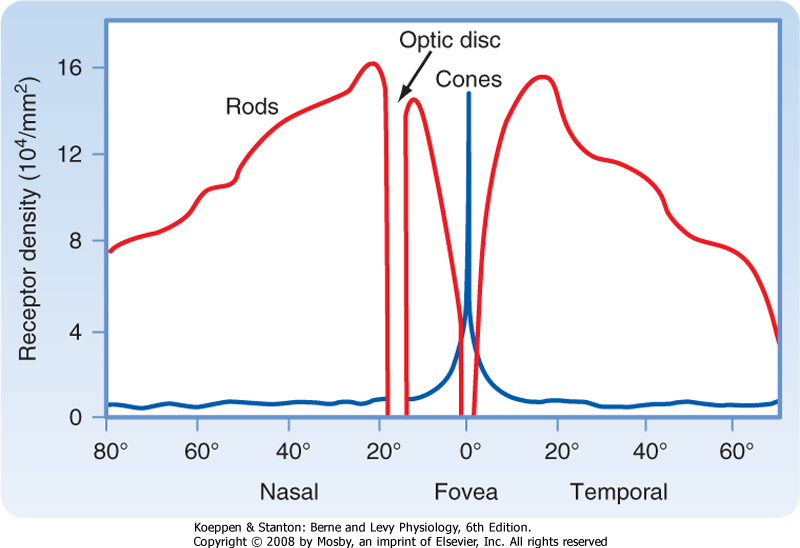
\includegraphics{rod_cone_density}
\caption{Plot of density of cones and rods against their angular distance from
the fovea. The cone density peak lies at the fovea, where there is an absence
of rods.\cite{rod_cone_density}}
\label{fig:rod_cone_density}
\end{figure}

The fovea has an apparent dip, because unlike the periphery, there are
no neurons situated behind it. Neurons are cells which process and
transmit electrical information. The cell body is connected to the optic
nerve through an extended nerve fibre, known as an axon, which sends
the visual information directly to the brain. As the photoreceptors (mainly
cones) beneath the fovea are responsible for the acuity and colour of the
centre field of vision, axons would disturb the tissue and result in a
distorted visual field.

A healthy and normal eye will pick up red, green and blue so that the
brain can interpret the full spectrum of colours. \Fref{fig:wavelengths}
shows normalised absorbance against wavelength for red, green and
blue cones and rods (which cannot differentiate between colours), in an
average, human eye. The range of human visual spectrum of light lies
roughly between 390nm and 700nm.\cite{starr2010biology}.

\begin{figure}[!htbp]
\centering
  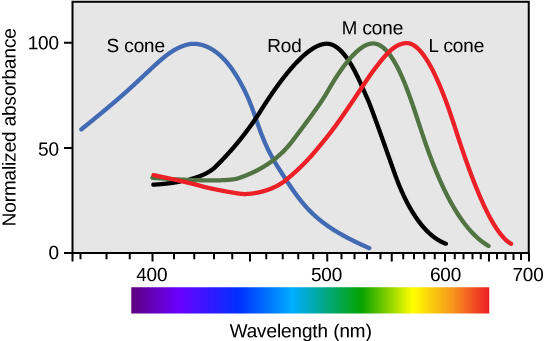
\includegraphics{wavelengths}
\caption{Normalised absorbance vs. wavelength, for cones of an average eye.\cite{wikicones}}
\label{fig:wavelengths}
\end{figure}

\section{Dysfunction in the Eye}

Unlike an ordinary optical system there exists the added complication
of common irregularities in patient vision such as myopia, astigmatism
or hyperopia. \Fref{fig:myop} demonstrates the optical effects of myopia,
a condition which occurs when the eyeball is shaped like a prolate oval.
\cite{saine2002ophthalmic} With myopia, light entering the eye is projected
in front of the retina instead of on its fovea so although the lens will be
accommodated so that nearby objects are in focus, this makes it difficult
for people to focus on far distant objects without the use of corrective
lenses.

\begin{figure}[htbp]
\centering
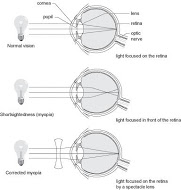
\includegraphics{figures/myopia}
\caption{An illustration of the visual effects of myopia and how it is corrected}
\label{fig:myop}
\end{figure}

When the eyeball is shaped like an oblate oval this can cause hyperopia,
a condition where light entering the eye is projected beyond the retina so
that it is difficult to focus on objects which are nearby without corrective
lenses.

Deviations from the model shape of an iris, for example when it is a conical
or oval-like shape, can cause a condition called astigmatism a condition which
can distort visual perception in a myriad of ways depending on the nature of
the irregularity of the iris.

As people age, ciliary muscles accommodating the lens weaken and
this also impairs their ability to focus on objects which are close by, this is
known as presbyopia. \cite{fisher1985ciliary}

A common defect affecting vision is often referred to as "colour blindness".
This is the limited functionality of certain cones which are are sensitive
to specific frequencies of light but not others such that a person can fail
to differentiate certain colours of the spectrum. This defect is related to
the X chromosome and hence it seems to only affect some men, who if
can be born with defected cones.\cite{george1996clinical} If all the cones
are defect, then this would result in blindness.

\section{Pathology of the Eye}

It is estimated that around two thirds of the incidents of blindness are those
which could be prevented with early diagnosis.\cite{west2000looking}
Approximately 16-20 million people are suffering from blindness due to
cataracts.\cite{west2000looking} The second most common cause of
blindness is trachoma, caused by the chlamydia infection, however it is
largely the developing world impacted with 5.9 million blinded by it
because in theory the disease can easily be treated by antibiotic drugs.
\cite{west2000looking}

Age related Macular degeneration (AMD) of pigment cells and
decreases in Equatorial rods and ganglion cell rates are common
problems affecting central vision.\cite{gao1992aging} AMD accounts
for 95\% of blind and partial sightedness registrations in the UK
and particularly affects women as well as the elderly.
\cite{o1998age,klein2005complement,west2000looking}
There are two main forms of AMD, non-exudative (dry) and exudative
(wet). The phenotypes in on-exudative AMD are atrophic and neovascular
respectively.\cite{kuno2011dry} In non-exudative macular degeneration,
deposits build up behind the retina resulting in its progressive thinning or
scarring, with respect to time. Exudative macular degeneration is caused
by leaking of blood vessels which causes swelling.

Preliminary studies indicate that the thickness of the choroid decreases
with age and although little is understood about how this may affect
central vision in macular degeneration, some studies have found
choroid thickness to be a predictor for open angle glaucoma which
is yet another leading cause of blindness.\cite{margolis2009pilot,gordon2002ocular}

Glaucoma is caused by various malfunctions of aqueous humour
drainage which can lead to excessive intraocular pressure bringing
about damage to the optic nerve and other vital members of the optical
system.\cite{distelhorst2003open} Open angle glaucoma happens
gradually, affecting the peripheral vision at first and progresses on to
impair central vision over time. For early diagnosis of open angle
glaucoma the relationship between intraocular pressure and visual
field decay is examined by specialists to determine whether any
abnormalities are apparent so that it may be treated before permanent
field damage occurs.\cite{goldmann1972open} Around 10\% of
glaucoma patients worldwide, go blind because of limited access to
preventative diagnosis and treatment.\cite{west2000looking}

Retinopathy is another common disease but one which can affect people of
all ages, by attacking the retina. A common indicator of non-proliferative
retinopathy is macular edema, symptomatic blurred vision arising from
abnormal fluid leakage and swelling in the macular from the retina's
blood vessels causing the the retina to thicken.\cite{hee1995quantitative}
Macular edema is the common cause of visual degeneration in people
with diabetes which can significantly increases a person's chance of
developing retinopathy as the diabetes progresses.\cite{klein1984wisconsin}
Proliferative diabetic retinopathy is caused by blockages in blood vessels
which can can starve the retina of oxygen. The retina responds to this by
attempting to grow blood vessels of its own, however they tend to be
abnormal and hinder fluid secretion and leak blood into the vitreous
humour. Symptoms of prolific retinopathy do not usually occur until
damage has already been done and in that case a sufferer would
experience seeing \enquote{floaters}, \enquote{shadows} and loss of vision.

\section{Eye Injury}

Common eye injuries are retinal detachment, corneal abrasions, exposure to
radiation and chemical burns. It has been estimated that 55 million eye injuries
occur each year worldwide and 1.6 million of those injuries result in complete
blindness.\cite{negrel1998global}

A UK study of 5671 eye patients in 1989 indicated that the incidence of
occupational eye injuries is around 69\%.\cite{macewen1989eye} A more
recent pilot study of eye injuries the UK suggests that \enquote{only} 31\%
of eye patients suffering from workplace injuries.\cite{thompson2009occupational}
The apparent improvement could be due to more strict regulations in health
and safety. Corneal injuries are relatively rare in the UK, with incidence at
0.02\%.\cite{macdonald2009surveillance}


